\subsection {Dise�o estructural}
A continuaci�n se muestra el diagrama de la arquitectura global de la aplicaci�n:

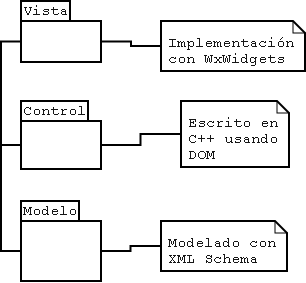
\includegraphics {figuras/png/Arquitectura.png}

La arquitectura MVC permite un desacoplamiento entre los distintos objetos que componen el sistema, permitiendo minimizar el impacto de los cambios entre capas del software. Adem�s, supone una arquitectura bien conocida, f�cil de entender, con riesgos calculados y que facilita la implementaci�n en un lenguaje dado, laportabilidad y las modificaciones.

Adem�s, la elecci�n de una arquitectura MVC no solo fomenta el desarrollo modular del programa sino que tambi�n expone claramente dicha modularidad, facilitando as� la comprensi�n del programa por parte de futuros desarrolladores. La estructura de dichos m�dulos se explicar� en subsiguientes p�rrafos.

El software se ha desarrollado como una aplicaci�n de escritorio 
monoproceso, pensada para ejecutarse en un entorno gr�fico. No se debe confundir la arquitectura MVC con las cl�sicas aplicaciones Web de 3 capas donde existen 3 procesos distintos que se ejecutan en tres nodos distintos a saber: El navegador Web que muestra la p�gina HTML, el servidor que atiende las peticiones HTML y de datos y el servidor de bases de datos que almacena y entrega los datos bajo petici�n del servidor Web. El programa tambi�n utiliza 3 capas, una de presentaci�n, una de l�gica de control y una de almacenamiento pero su prop�sito principal es la modularidad, y no la ejecuci�n separada de los distintos procesos.

A continuaci�n se muestran los componentes principales de cada capa:

Capa de Interfaz de usuario

Capa de control

Capa de modelo

Debido a la simplicidad de su arquitectura el despliegue de la misma no debe suponer ning�n problema, al haberse pensado la misma para construir un �nico programa ejecutable dependiente de algunas bibliotecas y que se ubicar� mediante un instalador en el directorio seleccionado por el usuario. En el manual de uso se describir� m�s ampliamente el proceso de despliegue. Las distintas capas de esta arquitectura han presentado ciertos problemas a la hora de su desarrollo ya que algunos problemas no se conoc�an en las etapas iniciales, como por ejemplo la integraci�n entre los distintos tipos de cadena de caracteres que ofrecen las distintas bibliotecas usadas al codificar.

La integraci�n de nuevos componentes 



